\documentclass[tikz]{standalone}
\usepackage{xcolor}
\definecolor{bg}{HTML}{171D2B}
\definecolor{acc}{HTML}{F7B538}
\pagecolor{bg}
\begin{document}
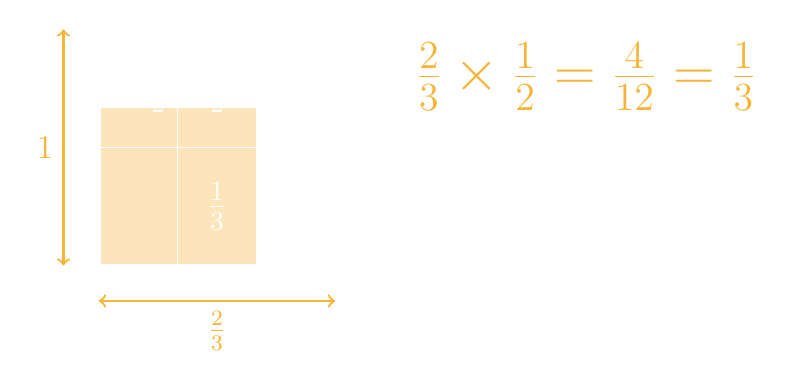
\begin{tikzpicture}[scale=1.0]
  % Unit square: 1/2 times 2/3
  \fill[acc, opacity=0.35] (0,0) rectangle (2,2);   % 2/3 wide, 1/2 tall -> 4/12
  \draw[white, very thick] (0,0) rectangle (3,3);
  % vertical thirds
  \foreach \x in {1,2} \draw[white] (\x,0) -- (\x,3);
  % horizontal halves
  \foreach \y in {1.5} \draw[white] (0,\y) -- (3,\y);
  % labels
  \node[white, font=\Large\bfseries] at (1.5,0.75) {$\frac{1}{3}$};
  \node[white, font=\Large\bfseries] at (2.5,0.75) {$\frac{1}{3}$};
  \node[white, font=\Large\bfseries] at (0.75,2.25) {$\frac{1}{2}$};
  \node[white, font=\Large\bfseries] at (2.25,2.25) {$\frac{1}{2}$};
  \node[white, font=\Large\bfseries] at (1.5,2.25) {$\frac{1}{2}$};
  % dimension arrows
  \draw[acc, <->, thick] (0,-0.45) -- (3,-0.45) node[midway, below, acc, font=\large] {$\frac{2}{3}$};
  \draw[acc, <->, thick] (-0.45,0) -- (-0.45,3) node[midway, left, acc, font=\large] {$1$};
  % result
  \node[acc, font=\huge\bfseries, anchor=west] at (3.9,2.4) {$\frac{2}{3} \times \frac{1}{2} = \frac{4}{12} = \frac{1}{3}$};
  \node[white, font=\large, anchor=west, text width=4.2cm] at (3.9,1.2)
    {4 dari 12 kotak kecil berwarna kuning};
\end{tikzpicture}
\end{document}
